% Encoding: UTF-8
% Build with: pdflatex
% Bibliography engine: bibtex8
% Should be a minimal set of packages and syntax bloat to be able to convert to HTML, RTF etc

\documentclass[a4paper,10pt,oneside,unicode]{article}
\usepackage[top=2cm,left=2.5cm,right=2cm,bottom=3cm]{geometry}
\usepackage[T2A]{fontenc}
\usepackage[utf8]{inputenc}
\usepackage{amsfonts}
\usepackage{amsmath}
\usepackage{amssymb}
\usepackage[english]{babel} % no Russian
\usepackage[pdftex]{graphicx}
\usepackage[pdftex]{hyperref}
\usepackage{indentfirst}

\hypersetup{colorlinks=true, linkcolor=black, filecolor=black, urlcolor=black,pdfauthor=Grigory Rechistov <grigory.rechistov@phystech.edu>,pdftitle=Simulation of CPUID of Intel Architecture}

% Extra fancy packages go here
\usepackage{bytefield}

\usepackage{tikz}
\usetikzlibrary{shapes, calc, arrows, fit, positioning, decorations, patterns, decorations.pathreplacing, chains}

\author{Grigory Rechistov\thanks{Moscow Institute of Physics and Technology, \texttt{grigory.rechistov@phystech.edu}} \and Name Surname\thanks{\texttt{email@mail.com}}}
\title{Simulation of CPUID of Intel Architecture}
\date{\today}

\newcommand{\cpuid}{\textsc{cpuid} }
\newcommand{\cpuidgen}{\textsc{cpuidgen} }

\newcommand{\todo}[1][]{\textcolor{red}{TODO #1}}
\newcommand{\othercopyright}{\textsuperscript{*}}
\begin{document}

\maketitle

\tableofcontents

\begin{abstract}
    
   \noindent In this paper we give an overview of existing microprocessor features identification facilities. Then we describe our approach to implementation of a software model of Intel IA-32 \cpuid instruction. The described solution allows to define all recent {CPUs}' features, as well as future extensions. Our model was incorporated into the Wind River Simics\othercopyright simulator framework.
    
    \noindent Key words: cpu identification, cpu simulation, CPUID, Simics.
\end{abstract}

\section {Introduction}

Most of documents defining CPU architectures do not specify every implementation detail; only interfaces, such as register state and instruction set (ISA), are defined. Microarchitectural details are usually left to vendors.

Any more-or-less mature processor architecture will have a set of extensions meant to improve performance, reliability, energy consumption or any other aspect of computer operation. A long evolution happened with backwards compatibility in mind and influenced by strong market competition will lead to a situation when there are quite a few of extensions, sometimes contradicting each other but nevertheless designated as “compatible” architectures.

Software programmers, who wish to use a certain architecture extension in their code, should be able to reliably identify its presence at run time. Therefore, processors provide means of feature identification in forms of instructions and/or registers which, being accessed, yield values that encode extended capabilities: vendor name, model name, machine word width, register count and similar model specific information.

Software simulators serve needs of pre-silicon software development, system firmware debugging, architecture and algorithm exploration etc. As with hardware, in order to be useful, software embodiments of processor specifications must faithfuly declare supported extensions. Yet, building a software model for processor feature identification may turn out to be a non-trivial task, complicated by a bulk and complexity of information that needs to be represented, especially when a number of supported processor models is high. 

From our experience with pre-silicon simulation tools, certain types of target software, such as BIOS, firmware and drivers, are quite sensitive to processor identification and will refuse to work or crash if a single bit of it is wrong. At the same time, such software in its early age may be incomplete; a software model has to adapt to mimic features that are absent for it to work. A naïve ad-hoc approach to feature data storage and handling will lead to a code that is very hard to extend support. These circumstances lead us to develop a dedicated framework for simulation of \cpuid instruction, described in the paper.

The rest of this paper is organized as follows. In the section~\ref{sec:overview}, we present a survey of approaches to defining model-specific features used in different microprocessor architectures. In the section~\ref{sec:ia-32-cpuid} it is shown that the Intel IA-32 has one of the most complex \cpuid instruction. Section~\ref{sec:approaches} describes approaches to \cpuid representation and simulation found in several software models. A new specification language for \cpuid definition and tools for generation of simulation code are described in section~\ref{sec:cpuidgen}. Our experience with its integration  into an industrial simulation framework Wind River Simics\othercopyright are shown in section~\ref{sec:evaluation}. Section~\ref{sec:conclusions} gives final remarks and future work directions.

\subsection{Contributions}

In this paper we make the following contributions.
\begin{enumerate}
\item Comparison of existing approaches to extensions/feature identification of different modern processor architectures. To our knowledge, no such survey has been published yet.
\item Describe design, implementation and evaluation of a structured solution to the simulation of \cpuid instruction of Intel IA-32. Analysis of several open source and proprietary simulators has shown that \cpuid simulation is traditionally made ad-hoc, resulting in an entanglement of code which is hard to support.
\item Define essential user interface facilities that firmware developers demand from a \cpuid simulation. We describe how \cpuid should be represented for inspection, and what types of manupulation should be allowed to an end user.
\end{enumerate}

\section{Overview of Processor Identification}\label{sec:overview}

This section outlines mechanisms for processor identification employed by several modern general purpose microprocessor architectures. We do not attempt to give exhaustive descriptions of instruction sets; nor we intend to give a historical overview of now discontinued designs. The goal is to highlight differences and similarities between systems. Detailed explanations for all mentioned registers and instructions can be found at respective reference manuals cited below.

\subsection{MIPS}

MIPS CPUs store processor identification within PRid register, which is the 15\textsuperscript{th} register in Coprocessor~0~\cite{mips-arch}. It contains 32 bits of information (Fig.~\ref{fig:mips-prid}), part of which is vendor--specific.

\begin{figure}[htbp]
\bytefieldsetup{bitwidth=0.36cm, endianness = big}
\centering
\begin{bytefield}[]{32}
    \bitheader{31,24,23,16,15,8,7,0} \\
    \bitbox{8}{Company Options} & \bitbox{8}{Company ID} & \bitbox{8}{Processor ID} & \bitbox{8}{Revision}
\end{bytefield}
\caption{MIPS PRid register fields}\label{fig:mips-prid}
\end{figure}

MIPS architecture also implements special register that contains information to list capabilities of floating point unit, termed Floating Point Implementation Register (FIR)~\cite{mips32-vol1}. It is a read-only 32-bit register (Fig.~\ref{fig:mips-fir}).

\begin{figure}[htbp]
\bytefieldsetup{bitwidth=0.5cm, endianness = big}
\centering
\begin{bytefield}[]{32}
    \bitheader{31,28,27,24,23,22,21,20,19,18,17,16,15,8,7,0} \\
    \bitbox{4}{00000} & \bitbox{4}{Impl} & \bitbox{1}{0} & \bitbox{1}{\footnotesize F64} & \bitbox{1}{L} & \bitbox{1}{W} & \bitbox{1}{3D} & \bitbox{1}{PS} & \bitbox{1}{D} & \bitbox{1}{S} & \bitbox{8}{ProcessorID} & \bitbox{8}{Revision}
\end{bytefield}
\caption{MIPS FIR register fields}\label{fig:mips-fir}
\end{figure}

\todo{Check this}

\url{http://hwdb.mipt.cc/MIPS_PRId_register}

\url{http://code.google.com/p/phantomuserland/source/browse/trunk/phantom/dev/mips/cpuid.c?r=1094}

\url{http://www.imgtec.com/mips/mips32-architecture.asp}

\subsection{ARM}

The popular RISC architecture ARM provides two different ways to identified cores. This ways described in~\cite{arm-application-note99}.

The first way is to read info form the Register 0 of the System Control Coprocessor also called \cpuid base register~\cite{arm-cpuid}. As with MIPS, it holds 32 bits of information and look a bit differ for ARM7 core family (Fig.~\ref{fig:arm-cpuid-v7}) and ARM9 and later core families (Fig.~{fig:arm-cpuid-v9}).

\begin{figure}[htbp]
\bytefieldsetup{bitwidth=0.36cm, endianness = big}
\centering
\begin{bytefield}[]{32}
    \bitheader{31,24,23,22,16,15,4,3,0} \\
    \bitbox{8}{Implementer} & \bitbox{1}{A} & \bitbox{7}{Variant} & \bitbox{12}{Primary Part No} & \bitbox{4}{Revision}
\end{bytefield}
\caption{ARM7 Core Family \cpuid{} base register fields}\label{fig:arm-cpuid-v7}
\end{figure}

\begin{figure}[htbp]
\bytefieldsetup{bitwidth=0.36cm, endianness = big}
\centering
\begin{bytefield}[]{32}
    \bitheader{31,24,23,20,19,16,15,4,3,0} \\
    \bitbox{8}{Implementer} & \bitbox{4}{Variant} & \bitbox{4}{Arch.} & \bitbox{12}{Primarily Part No} & \bitbox{4}{Revision}
\end{bytefield}
\caption{ARM9 and later Core Family \cpuid{} base register fields}\label{fig:arm-cpuid-v9}
\end{figure}

Examples of values~\cite{xda-arm-id}: Intel (XScale) PXA272 -- 0x69054117, Qualcomm MSM7200A --- 0x4117b362.

The other way that ARM core can be identified is through a TAP ID~\cite{arm-application-note99} that used ton configure debug software and indicates the information about an ARM core.

\subsection{IBM System z}

IBM System z10~\cite{ibm-system-z10} provides \texttt{STSI} and \texttt{STIDP} instructions to obtain processor information.

The \texttt{STSI} instruction used to determine processor model and model capacity identifier for the base configuration and for any additional changes through update actions (Fig.~\ref{fig:systemz-stsi}).

\newcommand{\memsection}[5]{%
    % define the height of the memsection
    \bytefieldsetup{bitheight=#3\baselineskip}%
    \bitbox[]{4}{%
        \texttt{#1}% print end address
        \\
        % do some spacing
        \vspace{#3\baselineskip}
        \vspace{-2\baselineskip}
        \vspace{-#3pt}
        \texttt{#2}% print start address
    }%
    \rlap{\bitbox{28}{\color{#5}\rule{\width}{\height}}}%
    \bitbox{28}{#4}% print box with caption
}

\begin{figure}[htbp]
\centering
\begin{bytefield}{32}
    \memsection{16}{}{4}{Model Capacity Identifier}{gray} \\
    \memsection{20}{}{4}{Sequence Code}{white} \\
    \memsection{24}{}{1}{Plant of Manufacture}{white} \\
    \memsection{25}{}{4}{Model}{white} \\
    \memsection{29}{}{4}{Model-Permanent-Capacity Identifier}{gray} \\
    \memsection{33}{}{4}{Model-Temporary-Capacity Identifier}{gray} \\
    \memsection{37}{}{1}{Model-Capacity Factor}{white} \\
    \memsection{38}{}{1}{Model-Permanent-Capacity Factor}{white} \\
    \memsection{39}{}{1}{Model-Temporary-Capacity Factor}{white} \\
    \memsection{40}{1023}{4}{Reserved}{white} \\
\end{bytefield}
\caption{\texttt{STSI} output}\label{fig:systemz-stsi}
\end{figure}

The \texttt{STIDP} instruction provides information about the processor type, serial number, and logical partition identifier (Fig.~\ref{fig:systemz-stidp}).

\begin{figure}[htbp]
\bytefieldsetup{bitwidth=0.25cm, endianness = big}
\centering
\begin{bytefield}[]{64}
    \bitheader{63,48,47,32,31,8,7,0} \\
    \bitbox{16}{Logical partition 2-digit indicator} & \bitbox{16}{Machine type number} & \bitbox{24}{CPU identification number} & \bitbox{8}{Version code}
\end{bytefield}
\caption{\texttt{STIDP} output}\label{fig:systemz-stidp}
\end{figure}

\subsection{PowerPC}

PowerPC~\cite{powerpc64-arch} offers a 32-bit PVR register that contains just version and revision numbers.

For ISA extensions a mechanism of APU (application processor units) is employed. MSR (machine state register) is used to store information of APUs available.

\todo{See also}

\url{http://lxr.linux.no/#linux+v3.13.5/arch/powerpc/kernel/cputable.c#L2245} --- identify\_cpu function

\url{http://cache.freescale.com/files/archives/doc/support_info/PPCPVR.pdf}

\subsection{SPARC}

The SPARC~v9 standard~\cite{weaver1994sparc} leaves quite a number of details implementation specific. To distinct between version a 64-bit register VER is defined (Fig.~\ref{fig:sparc-ver}).

\begin{figure}[htbp]
\bytefieldsetup{bitwidth=0.25cm, endianness = big}
\centering
\begin{bytefield}[]{64}
    \bitheader{63,48,47,32,31,24,23,16,15,8,7,5,4,0} \\
    \bitbox{16}{Manufacturer} & \bitbox{16}{Implementation} & \bitbox{8}{Revision} & \bitbox{8}{---} & \bitbox{8}{\footnotesize{Max trap levels}} & \bitbox{3}{---} & \bitbox{5}{\footnotesize{Max window}}
\end{bytefield}
\caption{SPARC~v9 VER register fields}\label{fig:sparc-ver}
\end{figure}

\subsection{Intel IA-64 (Itanium)}

Intel IA-64, also known as Itanium\texttrademark~\cite{itanium-sdm} was conceived after the original Intel 80x86 series and was meant to supplant it. A set of \cpuid registers is used for identification purposes. The set's design somewhat resembles IA-32 \cpuid instruction (discussed shortly after) --- its register numbers loosely resemble leaves of the latter. At the moment of this writing, all announced IA-64 systems offered up to five \cpuid registers. To have room for feature expansion, bits 0--7 of \textsc{cpuid[3]} store the actual size of the register set (limiting it to 256 entries).

A \cpuid table for an Itanium 2 system is given on Fig.~\ref{fig:itanium-cpuid}. Total capacity of it can be estimated as $5 \times 64 = 320$ bits.

\begin{figure}[htbp]
    \centering
\begin{verbatim}
Leaf              Value
-----------------------
  0  0x49656e69756e6547
0x1          0x6c65746e
0x2                   0
0x3          0x20010104
0x4                 0x5
\end{verbatim}
    
\caption{Contents of \cpuid registers for an Intel Itanium 9100 (code name Montvale) system using \texttt{ggg-cpuid}~\cite{ggg-cpuid}}\label{fig:itanium-cpuid}
\end{figure} 

% Result of cat /proc/cpuinfo on the Itanium host:
% processor  : 7
% vendor     : GenuineIntel
% arch       : IA-64
% family     : Itanium 2
% model      : 1
% revision   : 1
% archrev    : 0
% features   : branchlong, 16-byte atomic ops
% cpu number : 0
% cpu regs   : 4
% cpu MHz    : 1668.000672
% itc MHz    : 416.667500
% BogoMIPS   : 3325.95
% siblings   : 2
% physical id: 196867
% core id    : 1
% thread id  : 0
%
%uname -a
% Linux host 2.6.18-164.el5 #1 SMP Tue Aug 18 15:54:55 EDT 2009 ia64 ia64 ia64 GNU/Linux
% lsb_release -a
% LSB Version:    :core-3.1-ia64:core-3.1-noarch:graphics-3.1-ia64:graphics-3.1-noarch
% Distributor ID: RedHatEnterpriseServer
% Description:    Red Hat Enterprise Linux Server release 5.4 (Tikanga)
% Release:        5.4
% Codename:       Tikanga


% The \texttt{mov =cpuid[...]} instruction is defined to read a processor identification information.

\subsection{Intel IA-32 and Intel 64}

The common IBM PC architecture, starting from Intel Pentium\texttrademark and its clones, provides \cpuid instruction~\cite{intelmanual-7vols, amd-sdm-vol1}. The 64-bit extension of IA-32, known as Intel~64 or AMD64, did not change \cpuid and we will make no further distinction between them throughout this paper. and we will make no distinction between them. \cpuid takes two input operands in 32-bit registers EAX and ECX (called \textit{leaf} and \textit{subleaf}) and puts the result to four 32-bit registers, namely EAX, EBX, ECX and EDX.

Since its inception it has been extended numerous number of times.\todo{Expand}

On Figure~\ref{fig:x86-cpuid} an output of all defined leaves and subleaves for a modern Intel processor (of microarchitecture Intel Ivy Bridge) is shown. The resulting table contains 25 tuples of 4 values of 32 bit width each, total of more than 3 kbit of information. Essentially a number of features can be deduced from it.
\begin{itemize}
    \item Processor producer brand (leaf 0) and SKU naming (leaves 0x80000002--0x80000004).
    \item Availability of ISA extensions such as 64 bit mode, SSE2/3/4.1/4.2, AVX, MOVBE etc.
    \item Cache configuration of all layers, both in legacy format (leaf 2) and in current format (leaf 4 with subleaves).
    \item Multi-processor configuration knowledge, such as availability of Intel HyperThreading, relative position inside {CPU} package (topology at leaf 11), presence of {APIC} (interrupt controller).
    \item Numerous parameters for the implementation, such as addresses widths (leaf 0x80000008), availability of dynamic frequency scaling, supported debugging facilities etc.
\end{itemize}


\begin{figure}[htbp]
\centering
\begin{verbatim}
Leaf             Subleaf         EAX         EBX        ECX          EDX
------------------------------------------------------------------------
           0           0         0xd  0x756e6547  0x6c65746e  0x49656e69
         0x1           0     0x306a9   0x6100800  0x7f9ae3bf  0xbfebfbff
         0x2           0  0x76035a01    0xf0b0ff           0    0xca0000
         0x4           0  0x1c004121   0x1c0003f        0x3f           0
         0x4         0x1  0x1c004122   0x1c0003f        0x3f           0
         0x4         0x2  0x1c004143   0x1c0003f       0x1ff           0
         0x4         0x3  0x1c03c163   0x2c0003f      0x1fff         0x6
         0x5           0        0x40        0x40         0x3      0x1120
         0x6           0        0x77         0x2         0x9           0
         0x7           0           0       0x281           0           0
         0xa           0   0x7300803           0           0       0x603
         0xb           0         0x1         0x1       0x100         0x6
         0xb         0x1         0x4         0x4       0x201         0x6
         0xb         0x2           0           0         0x2         0x6
         0xb         0x3           0           0         0x3         0x6
         0xd           0         0x7       0x340       0x340           0
         0xd         0x1         0x1           0           0           0
         0xd         0x2       0x100       0x240           0           0
  0x80000000           0  0x80000008           0           0           0
  0x80000001           0           0           0         0x1  0x28100800
  0x80000002           0  0x20202020  0x20202020  0x65746e49  0x2952286c
  0x80000003           0  0x726f4320  0x4d542865  0x35692029  0x3534332d
  0x80000004           0  0x50432030  0x20402055  0x30312e33    0x7a4847
  0x80000006           0           0           0   0x1006040           0
  0x80000007           0           0           0           0       0x100
  0x80000008           0      0x3024           0           0           0
\end{verbatim}

    \caption{Output of \cpuid instruction obtained for Intel\textregistered{} Core\texttrademark{} i5-3450 using \texttt{ggg-cpuid}~\cite{ggg-cpuid}}\label{fig:x86-cpuid}
\end{figure}

\subsection{Comparison of Processor Identification}

Based on the presented data several conclusions can be made.
\begin{itemize}
    \item {CPU} identification facilities differ greatly between architectures. They may be represented by instructions, registers, or groups of both.
    \item The common thing that is usually conveyed through a \cpuid is a vendor identification. The next on popularity is indication of ISA extensions. Lastly, for multiprocessor systems, values for enumerating cores, threads or processors is often given.
    
    \item The “verbosity” of \cpuid facilities depends on whether there are requirements to run the same binary code on hardware from multiple vendors and/or of different generations. If, in order to perform efficiently, software must “know” a list of supported instruction extensions and other types of model specific configuration, there has to be a documented way to obtain such knowledge.
    \item Conversely, {CPUs} provided by a single vendor and/or designed for specific software usually provide less means of self-identification. Most microcontrollers for embedded applications hardly provide even an idea of \cpuid, compared to general purpose processors, because software is often written to be run on a specific HW; binaries are not meant to be moved to some other incarnation of the same architecture.
    
%     \item It is basically hard to define completely what identification facilities should store.
\end{itemize}

\section{What is so Hard about IA-32 CPUID}\label{sec:ia-32-cpuid}

We now concentrate solely on the Intel IA-32 architecture and its \cpuid. The previous section demonstrates that this instruction generates significantly more data than any other identification mechanism of the rest of surveyed systems. Indeed, a complete definition of \cpuid in~\cite{intelmanual-7vols} takes about 40 pages. 

\subsection{Subleaves, Dynamic Fields and Topology}

Let's go through all the complications of \cpuid that have to be modeled in a software simulator.

\paragraph{Elements adressing.} An “address” of a particular extension field inside a \cpuid table comprises of four values.

\begin{itemize}
\item Leaf number. It's the input value of EAX for \cpuid invocation. There are two continuos numerical ranges for leaf values: the first starting from zero and the second starting from 0x80000000 (see Fig.~\ref{fig:x86-cpuid}).
\item Subleaf number. An input value of ECX for \cpuid invocation. Only a few leaves actually have a non-zero number of subleaves; for example, leaf 4 uses them to distinct between cache levels. For the rest, the subleaf is ignored and the instruction's output does not depend on it.
\item Output register. Execution of \cpuid always changes four registers, effectively producing a 128-bit value. The register name is specified to choose a 32 bit range inside it.
\item Bit range. A field can occupy from one to 32 bits of an output register.
\end{itemize}

In order to fully specify placement of a \cpuid field, all these values must be known. For example, the following notation is used in documentation to denote presence of MMX technology: \texttt{CPUID.01H:EDX.MMX[bit 23]}.

% The non-regularity of leaf--subleaf structure has to be reflected in the model.

\paragraph{Dynamic fields.} Firmware can affect output of \cpuid by enabling and disabling architectural extensions. Let's have some examples.
\begin{enumerate}
    \item Disabling multiple cores and Intel HyperThreading technology affects the CPUID.1:EDX.HTT[28].
    \item Changing bit 18 of register CR4 affects CPUID.1:ECX.OSXSAVE[27].
    \item A number of bits in the IA32\_MISC\_ENABLE model specific register affect \cpuid. Thus, its bit 16 affects indication of EIST field, bit 34 disables Execute Disable feature and its indication in \cpuid etc.
\end{enumerate}

These facts mean that one cannot just use a constant array to represent the table in the simulation --- some bits will be dynamic and have to be calculated every time an instruction is run.

\paragraph{Topology-variable elements.} In multiprocessor systems different processor cores inside the same CPU package will have \cpuid returning different values, because certain fields indicate relative position of them (topology). For example, the 8-bit of APIC ID of a core is returned in CPUID.1.EBX[24:31]. This means that for simulation we cannot store a single table for all cores.

Finally, it should be noted that, besides EAX, EBX, ECX and EDX, one more register may be affected by \cpuid execution, namely IA32\_BIOS\_SIGN\_ID MSR.

\subsection{Why CPUID is so complex}

One can find roots of having such entangled (and nonsurprisingly slow) instruction by studying the history of IA-32 architecture.
\paragraph{Influence of multiple competing vendors.} Until recently, there were numerous {CPU} vendors that offered processors compatible with Intel architecture, including IBM, Cyrix, VIA, Centaur, Transmeta etc. By 2014, considerably fewer companies remain --- in particular Intel itself and AMD. A coordination committee to define how new IA-32 extensions are indicated have not existed. Uncontrolled competition lead to the numerous small and subtle but essential differences in implementation. 
Until (and for some time after) \cpuid was introduced, a robust identification of IA-32 processor brand and model required surprisingly intricate methods~\cite{cpuid-wars}. At present times, things are somewhat better documented, but still are not controlled in a centralized manner.

\paragraph{Long history that lead to extremely long list of extensions.} With 40 years of backwards-compatible development the IA-32 architecture collected a number of additions. Consider a list of flags which a modern GNU/Linux operating system shows for a \cpuid of the laptop this paper is being written on (Fig.~\ref{fig:flags}). It should be noted that only a part of information from \cpuid is actually present on this list.

\begin{figure}
\noindent\texttt{flags           : fpu vme de pse tsc msr pae mce cx8 apic sep mtrr pge mca cmov pat pse36 clflush dts acpi mmx fxsr sse sse2 ss ht tm pbe syscall nx rdtscp lm constant\_tsc arch\_perfmon pebs bts nopl xtopology nonstop\_tsc aperfmperf pni pclmulqdq dtes64 monitor ds\_cpl vmx est tm2 ssse3 cx16 xtpr pdcm pcid sse4\_1 sse4\_2 x2apic popcnt tsc\_deadline\_timer xsave avx lahf\_lm arat epb xsaveopt pln pts dtherm tpr\_shadow vnmi flexpriority ept vpid
}
\caption{Part of output of \texttt{cat /proc/cpuinfo} command on GNU/Linux on a recent Intel IA-32 {CPU}}\label{fig:flags}
\end{figure} 


\section{Existing Approaches to CPUID Simulation}\label{sec:approaches}

Every software simulator, emulator or virtual machine of a recent (Pentium or later) IA-32 system must guarantee \cpuid operation of certain accuracy. If such tool is used for system firmware development, which is even more sensitive to identification information, the following requirements should be.

\begin{itemize}
\item Be accurate \todo
\item Be configurable \todo
\end{itemize}

\subsection{Bochs}

Bochs~\cite{bochs} \todo 

\subsection{Xen}

Xen~\cite{xen2006} \todo *

\subsection{Qemu}

Qemu~\cite{qemu} \todo 

\subsection{Simics}

Wind River Simics~\cite{simics} \todo

\section{CPUID Definition and Generation}\label{sec:cpuidgen}

The approach to be described 

\subsection{Starting Considerations}

The following considerations have been taken into account when designing the specification.

\begin{itemize}
\item Have as much regular format as possible.
\item Use a natural unit of \cpuid configuration state --- a field.
\item Move computation tasks from run-time to the translator
\item Users often think and operate in terms of 32 bit register values which are more compact and therefore convenient.
\end{itemize}

\subsection{Specification of CPUID}
\paragraph{Fields definition.} This is a common part of all models. Here, the exact position, name, and properties of all fields are specified.

Types of the fields:
\begin{enumerate}
    \item const ---
    \item field ---
    \item fuse ---
    \item func --- 
\end{enumerate}

\paragraph{Model Definition.} For every CPU model a separate file section formulates what actual values for fields/fuses/func's the model should have. 

At model definition section, actual values are set up for all fields defined in the fields section.

A (shortened) example of an input specification is given at Fig.~\ref{fig:field-spec}.

\begin{figure}[htbp]
    \centering
\begin{verbatim}
[FIELDS]
# name    leaf sleaf  reg  range   type flags  defval       comment
  sse3,      1, None, ecx,     0, field,    0,      0,      Availability of SSE3
cache_descr, 1, None, eax,  0:31,  fuse,    0,   0x62,      Cache descriptor
apic_id,     1, None, ebx, 24:31,  func,    0, get_apic_id, APIC ID

[CPUID]
# class, field,      value
Atom,    sse3,       1
Atom,    logical_no, atom_apic_id
Atom,    4:1,        0x11111111:0x22222222:0x33333333:0x44444444

\end{verbatim}
\caption{Examples of fields and model definitions. Lines starting with “\#” are ignored}\label{fig:field-spec}
\end{figure}

\subsection{Translation to Code}

We implemented a translator called \cpuidgen that accepts a file with the specification outlined above and generates source code files, which are included into the build. Fig.~\ref{fig:workflow} outlines the process of integration of the new functionality with the rest of the simulation framework.

\begin{figure}[htbp]
\centering
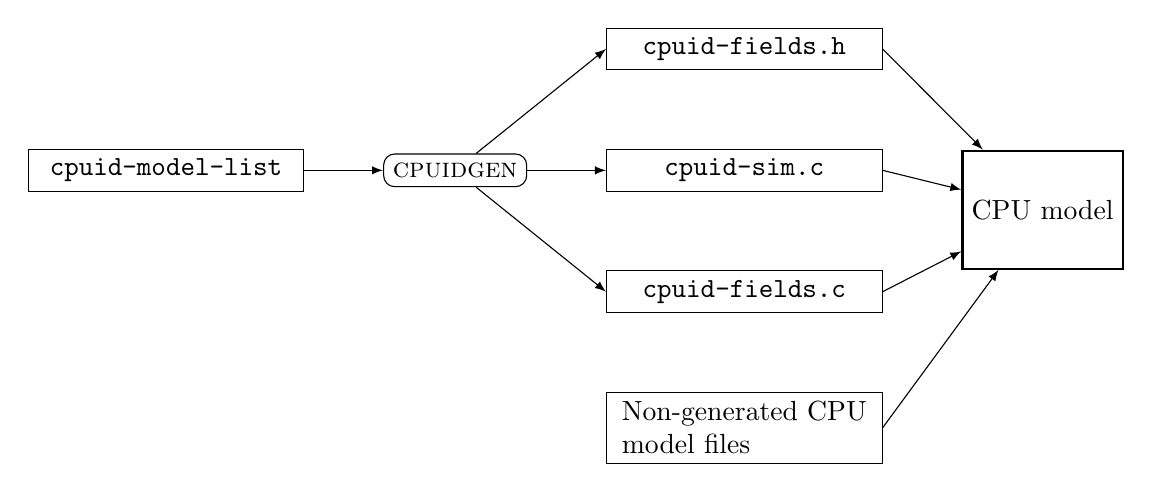
\begin{tikzpicture}[>=latex, minimum width = 3.5cm]
    \node[draw] (input) {\texttt{cpuid-model-list}}; 
    \node[draw, rounded corners, right = of input, minimum width = 1cm] (cpuidgen) {\cpuidgen};
    \node[draw, right = of cpuidgen] (cpuid-sim-func) {\texttt{cpuid-sim.c}}; 
    \node[draw, above = of cpuid-sim-func.north west, anchor=south west] (cpuid-headers) {\texttt{cpuid-fields.h}}; 
    \node[draw, below = of cpuid-sim-func.south west, anchor=north west] (cpuid-aux) {\texttt{cpuid-fields.c}}; 
    \node[draw, below = of cpuid-aux.south west, anchor=north west, align=left, ] (rest-src) {Non-generated CPU\\model files};
    \node[draw, thick, right = of cpuid-sim-func, minimum width = 1cm, minimum height=1.5cm, yshift=-0.5cm] (cpu-model) {CPU model};
    
    \draw[->] (input) -- (cpuidgen);
    \draw[->] (cpuidgen) -- (cpuid-sim-func.west);
    \draw[->] (cpuidgen) -- (cpuid-headers.west);
    \draw[->] (cpuidgen) -- (cpuid-aux.west);
    \draw[->] (cpuid-sim-func.east) -- (cpu-model);
    \draw[->] (cpuid-headers.east) -- (cpu-model);
    \draw[->] (cpuid-aux.east) -- (cpu-model);
    \draw[->] (rest-src.east) -- (cpu-model);
    
\end{tikzpicture}
\caption{Steps of building for a CPU model} \label{fig:workflow}
\end{figure} 

The build consists of these steps.
\begin{enumerate}
    \item \cpuidgen reads cpuid-model-list and produces three files: a C header with definitions of all structures and function prototypes, a C source for the main simulation function, \texttt{cpuid\_simulate()}, and C source for auxiliary functions.
    \item New sources are included, built and linked with the rest of the CPU model files.
\end{enumerate}

\subsection{Generated Code}

The \texttt{cpuid\_simulate()} is a C function that consists of two levels of \texttt{switch} operators --- the outer level is for leaf selection, and the inner --- for subleaf selection, if any subleaves are present. When leaf/subleaf combination is filtered out, all relavant CPUID fields are combined to create four 32-bit values of output registers. This allows to keep algorithmical complexitiy of the algorithm to be $O(1)$ of number of leaves and subleaves, and $O(N)$ of number of fields. The previous implementation performed a linear search for matches against input leaf/subleaf, which, of course, is less efficient. The translator shifts this search to the compilation time, thus saving run-time.

\section{Evaluation}\label{sec:evaluation}

\subsection{Compatibility with existing code}

“legacy” 

\subsection{Overriding Facilities}

\todo the picture of \cpuid dump with overridden fields highlighted.


\subsection{Extensions}

\todo Field flags, such as “hidden”.

\section{Conclusions}\label{sec:conclusions}

In this paper we described our approach to simulation of a single but complex processor instruction \cpuid. 

\paragraph{Model specific registers.} Besides \cpuid, processors of Intel architecture may have a quite extensive of model specific registers (MSRs), which can be read/written with \textsc{rdmsr/wrmsr} instructions, and also contain bits of processor identification. The simulation of MSRs is also an important aspect, but it is out of this paper focus. Other architectures may have similar facilities, e.g. special purpose registers (SPRs) in PowerPC. 

\section*{Acknowledgements}

Thanks to my parents for raising an awesome me.

\bibliographystyle{plain}
\bibliography{art} % use bibtex8, NO SPACES HERE!

\end{document}
